\subsection{Theoretical Analysis} \label{subsec:intro}

\begin{tcolorbox}	
\begin{tabular}{p{2.75cm} p{0.2cm} p{10.5cm}}
\textbf{Contributors}  &:& Nelson Muga (2017-12-20 - )\\
                       &:& Diamantino Silva (2017-08-18 - ...)\\
                       &:& Armando Pinto (2017-08-15 - ...)\\
\textbf{Goal}          &:& Theoretical description of various optical detection schemes.\\
\end{tabular}
\end{tcolorbox}

Receiver schemes for the detection of optical modulated signals can be roughly divided into two basic groups: Direct detection and coherent detection.   In a direct detection receiver, its photodiode only responds to changes in the receiving signal optical power, and cannot extract any phase or frequency information from the optical carrier. However, using direct detection along with additional optics, e.g. an interferometer, the phase in one symbol may be compared to the phase in the previous symbol. This is often called interferometric detection. Coherent receivers use a carrier phase reference generated at the receiver, i.e. a local oscillator, and  can track the phase of an optical transmitter so as to extract any phase and frequency information carried by a transmitted signal. Table~\ref{TAB_DetTech} compares the three detection techniques, including maximum number of degrees of freedom and receiver sensitivities for binary and quaternary modulations.

\begin{table}[h]\caption{COMPARISON OF DETECTION TECHNIQUES. SHADING DENOTES AN ADVANTAGE (from \cite{Kahn2004} and \cite{Kahn2006}).}\label{TAB_DetTech}
\centering
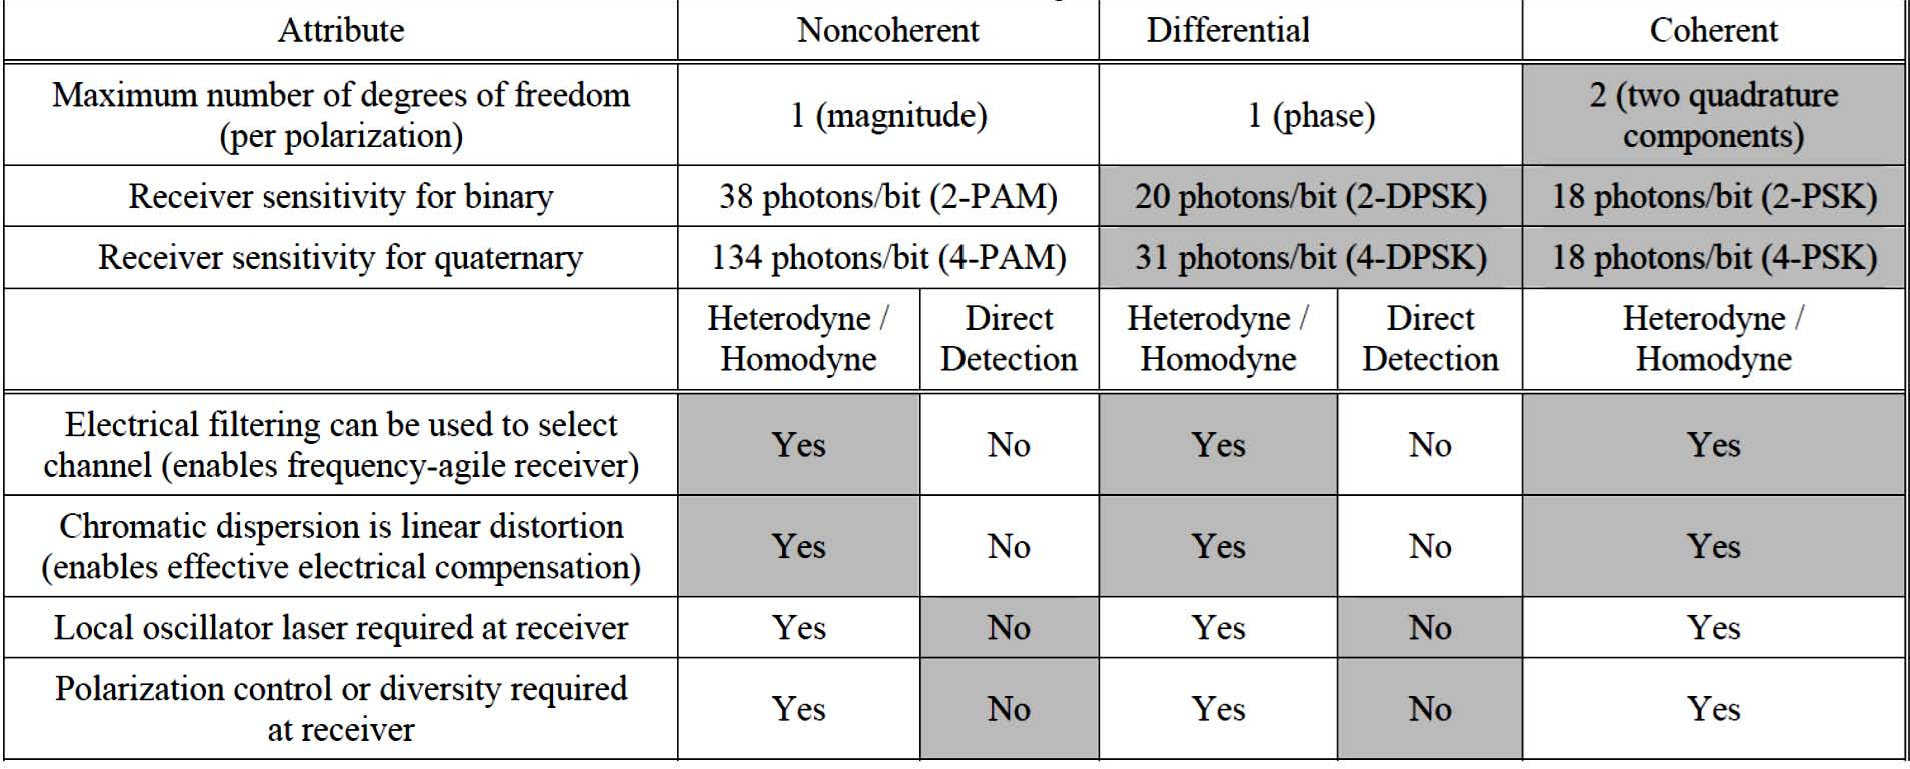
\includegraphics[width=6in]{./sdf/optical_detection/figures/Detection-Techniques-Kahn.pdf}
\end{table}



In this subsection, we are going to calculate the signal-to-noise ratio at the input of the decision circuit for the various detection schemes under analysis.
For each detection scheme a classical and a quantum description is going to be developed and a comparative analysis is going to performed.

\subsubsection{Classical Description}

\begin{tcolorbox}	
\begin{tabular}{p{2.75cm} p{0.2cm} p{10.5cm}}
\textbf{Contributors}  &:& Nelson Muga (2017-12-20 - )\\
                       &:& Diamantino Silva (2017-08-18 - ...)\\
                       &:& Armando Pinto (2017-08-15 - ...)\\
\textbf{Goal}          &:& Develop a classical description of various optical detection schemes.\\
\end{tabular}
\end{tcolorbox}

{\bf \em Direct Detection }\\

Direct detection schemes are convincingly simple as no phase, frequency or polarization control is necessary to recover the intensity of the optical field. This section will focus only the recover of the intensity of the optical field through the calculation of the current intensity at the output of a photodiode.


\begin{figure}[h]
	\centering
	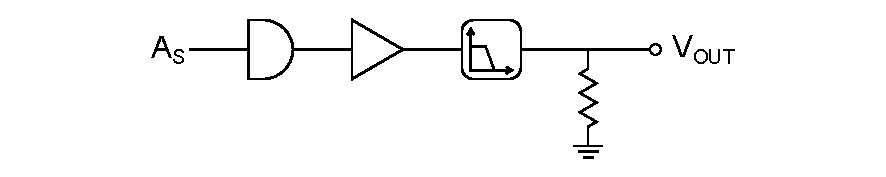
\includegraphics{./sdf/optical_detection/figures/detection-direct.pdf}
	\caption{Noncoherent detection technique with direct detection implementation.}\label{fig:detection_direct}
\end{figure}

\noindent


The electric field generated by an monochromatic single mode laser arriving at the input of the optical receiver can be written as

\begin{equation}\label{Eq_Ein}
    E_s(t)=\sqrt{P_s}\cdot A(t)\cdot e^{i(\omega_s t+\varphi_s)}
\end{equation}
where ${P_s}$ is the optical power, $\omega_s$ is the carrier frequency, $\varphi_s$ is the initial phase, and $A=a(t)e^{i\varphi(t)}$ is the modulated envelop amplitude, with $a(t)$ and $\varphi(t)$ standing for the modulated amplitude and phase, respectively.

The output current of the photodiode, $I_{DD}(t)$ can be written as
\begin{align}\label{Eq_Iout1}
    I_{DD}(t) &= R\cdot E_s(t)\cdot E^*_s(t)+i_{sh}+i_{th}\\
              &= R\cdot a^2(t)\cdot P_s+i_{sh}+i_{th},\label{Eq_Iout2}
\end{align}
where $R$ represents the responsivity of the photodiode, which is equal to
\begin{equation}\label{Eq_Responsivity}
    R = \eta\frac{2\pi q}{h\omega_s},
\end{equation}
with $q=1.6\cdot10^{-19}$~C being the charge of the electron, $h\omega_s/2\pi$ is the energy per photon with $h=6.63\cdot10^{-34}$~J$\cdot$s being the Planck constant, and $\eta$ is the fundamental quantum efficiency of the photodiode that corresponds to the averaged number of electrons generated per photon (Ref.Agrawal2013).

The two last terms on the right hand side of equation (\ref{Eq_Iout2}), $i_{sh}$ and $i_{th}$, represent the current fluctuation related to the shot noise and thermal noise effects, respectively. From the classical interpretation, the shot noise is induced by the optical-to-electrical conversion process. Mathematically, $i_{sh}(t)$ is a stationary random process with Poisson statistics, whose autocorrelation function is related with to the spectral density (Ref.Agrawal2012)

\begin{equation}\label{Eq_AC_i_sh}
    \left<i_{sh}(t)i_{sh}(t+\tau)\right> = \int_{-\infty}^{+\infty}S_{sh}(f)e^{i2\pi f\tau}df
\end{equation}
where $\left<\cdot\right>$ stands for the ensemble average over fluctuations. The two-sided spectral density (notice that the integral in (\ref{Eq_AC_i_sh}) includes both negative and positive frequencies) of the shot noise is a constant term and can be written as
\begin{equation}\label{Eq_SD_i_sh}
    S_{sh}(f)=q I_p
\end{equation}
where $I_p$ is the average output current of the photodiode presented in equation (\ref{Eq_Iout1}), i.e., 
\begin{equation}\label{Eq_I_p}
I_p(t) = I_{DD}(t) -(i_{sh}+i_{th}).
 \end{equation}
The shot noise variance can be calculated by setting $\tau=0$
\begin{equation}\label{Eq_Var_i_sh}
    \sigma^2_{sh} =  \left<i_{sh}(t)^2\right> = \int_{-\infty}^{+\infty}S_{sh}(f)df = 2 q I_p B
\end{equation}
where $B$ is the photodetector bandwidth.  The thermal noise term represented in (\ref{Eq_Iout2}) is related with the random thermal motion of electrons in the load resistor in the front end of the receiver, see~Fig.~\ref{fig:detection_direct}. Mathematically, this noise contribution is modeled as a stationary Gaussian random process with a two-sided spectral density approximately constant (ref.Agrawal), given by
\begin{equation}\label{Eq_SD_i_th}
    S_{th}(f)= 2 k_B T/R_L
\end{equation}
where $k_B$ is the Boltzmann constant, $T$ is the absolute temperature and $R_L$ is the load resistor. Considering a autocorrelation function given by (\ref{Eq_AC_i_sh}), with the subscripts $sh$ replaced by $th$, and setting $\tau=0$, the noise variance becomes
\begin{equation}\label{Eq_Var_i_th}
    \sigma^2_{th} =  \left<i_{th}(t)^2\right> = \int_{-\infty}^{+\infty}S_{th}(f)df = \frac{4 k_B T}{R} B.
\end{equation}
It is worth noticing that: a) de photodiode bandwidth appears on the expressions of both noise terms; b) in contrast with the shot noise case, the variance of the thermal noise does not depend on the average photocurrent $I_p$.

Since the shot and thermal noise are independent random processes with approximately Gaussian statistics, the total variance of the current fluctuations, $\Delta i= i_{sh}+i_{th}$, can be written as the sum of the individual variances presented in (\ref{Eq_Var_i_sh}) and (\ref{Eq_Var_i_th})
\begin{equation}\label{Eq_Var_i_sh}
    \sigma^2_{\Delta I_{DD}} =  \left<\Delta I_{DD}^2\right> = \left(2qI_p+\frac{4 k_B T}{R}\right) B
\end{equation}
Once obtained the variance of the photocurrent one can easily compute the signal-to-noise-ratio (SNR) of the optical receiver, which is a key parameter on the performance assessment of the device. The SNR of a electrical signal is defined as the ratio of the average signal power over the noise power, which leads to 
\begin{equation}\label{Eq_SNR_Idd}
    SNR=\frac{I_p^2}{\sigma^2_{\Delta I_{DD}}}
\end{equation}
Using (\ref{Eq_I_p}) and (\ref{Eq_Var_i_sh}) into the previous equation, one obtains the SNR as a function of the optical field impinging the photodiode
 \begin{equation}\label{Eq_SNR_Idd}
    SNR=\frac{R^2(a^2(t)\cdot P_s)^2}{\left(2qI_p+ 4 k_B T/R\right) B}
\end{equation}

\newpage

--$\veebar\veebar$
--$\veebar\veebar$
--$\veebar\veebar$
--$\veebar\veebar$
--$\veebar\veebar$
--$\veebar\veebar$--

We will consider that the detector has a bandwidth $B$, greater that the signal $A(t)$, but much smaller than $2 \omega_0$. The calculation of power incident in the photodiode is given by the expected value of the square of the amplitude during a time interval $\Delta t = 2 \pi / \omega$\\

Measurable optical power, assuming that the detector bandwidth, $B$, is greater than the signal, $A(t)$, bandwidth but much small than $2 \omega_0$

\begin{align}
	P(t)	&= \overline{E_R^2(t)}\nonumber\\
			&= \overline{|A(t)|^2} + \overline{ |A(t)|^2 cos\left(-2 \omega t + 2\theta(t)\right)}\nonumber\\
         &= |A(t)|^2 \,\,\,\, W
\end{align}


\vspace{2em}
\noindent
To simplify calculations, the electric field can be expressed the complex notation
%
\begin{equation}
	E(t) = A(t) e^{-i \omega_0 t}
\end{equation}
%
%
The physically measurable quantities are obtained by taking the real part of the complex wave. Using this notation, the beam power, $P(t)$, is obtained by multiplying the electric field's conjugate by itself

\begin{align}
	P(t) &= E^{*}(t) E(t)\nonumber\\
         &= |A(t)|^2
\end{align}

\begin{equation}
	i(t) = \eta q \frac{P(t)}{\hbar \omega_0}
\end{equation}
in which $\eta$ is the photodiode's responsivity, q is the unit charge and $P(t)/\hbar \omega_0$ is the number of removed electrons.


which will use to express the second moment of the photocurrent as
\begin{equation}
	\langle i^2(t) \rangle = \eta^2 q^2 \frac{\langle |A(t)|^4 \rangle }{\hbar^2 \omega_0^2}
\end{equation}
Assuming a fase modulation, in which the amplitude is constant, the signal is simplified to
\begin{equation}
	A(t) = |A| e^{i \theta}
\end{equation}
Therefore, the current becomes constant
\begin{equation}
	i(t) = I_0 = \eta q \frac{A_s^2}{\hbar \omega_0}
\end{equation}
and it's second moment becomes simply
\begin{equation}
	\langle i^2(t) \rangle = I_0^2
\end{equation}

Shot noise in photodiodes\\

\begin{equation}
	\langle i_n^2(t) \rangle = 2 q B I_0
\end{equation}

The signal to noise ratio is obtained by the relation between the second moment of the sinal to the second moment of the noise

\begin{align}
	\frac{S}{N} &= \frac{\langle i^2(t) \rangle}{\langle i_n^2(t) \rangle} \nonumber\\
                &= \frac{I_0}{2 q B}\nonumber\\
                &= \eta \frac{ |A|^2}{\hbar \omega_0 B}
\end{align}

{\bf \em Homodyne Detection}\\

\begin{figure}[H]
	\centering
	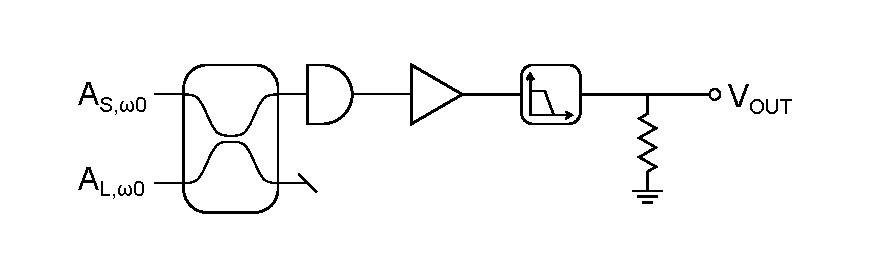
\includegraphics{./sdf/optical_detection/figures/detection-homodyne.pdf}
	\caption{Homodyne detection.}
\end{figure}
%%



The homodyne detection scheme uses an auxiliary local oscillator, which is combined in
a beamsplitter with the signal beam. After this step, it is similar to the direct detection. As we will see this has some implications in the phase detection???\\
\\
Given a splitter with intensity transmission $\epsilon$, the resulting field incident to the photodetector is
\cite{shapiro1985quantum} %p.241
%
\begin{equation}
	E(t) = \sqrt{\epsilon}E_S(t) + \sqrt{1-\epsilon}E_{LO}(t)
\end{equation}
%
in which $E_{LO} = e^{i \omega_0 t}$.
Given a local oscillator with a much larger power that the signal, then, the incident power in the photodiode is
%
\begin{align}
	P(t)	&= \eta \left[ (1-\epsilon) P_{LO}(t) + 2 \sqrt{\epsilon (1-\epsilon)} \textrm{Re} \left[ E_S(t) E^\ast_{LO}(t) \right] \right]\\
			&= \eta \left[ (1-\epsilon) P_{LO}(t) + 2 \sqrt{\epsilon (1-\epsilon)} |E_S(t)| |E_{LO}(t)| \cos{(\phi)} \right]\\
\end{align}

{\bf \em Balanced Homodyne Detection}\\
%
%

\begin{figure}[H]
	\centering
	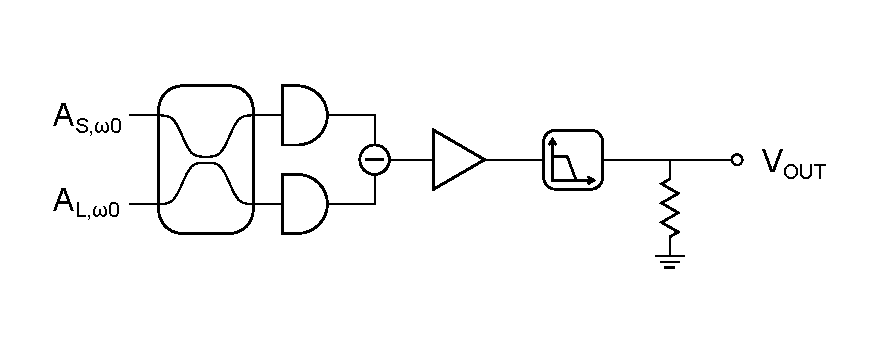
\includegraphics{./sdf/optical_detection/figures/detection-balanced-homodyne.pdf}
	\caption{Balanced homodyne detection.}
\end{figure}
%%
"In a balanced homodyne detector (BHD), the signal to be measured is mixed with a local oscillator (LO) at a beam splitter. The interference signals from the two output ports of the beam splitter are sent to two photodiodes followed by a subtraction operation, and then, amplification may be applied. The output of a BHD can be made to be proportional to either the amplitude quadrature or the phase quadrature of the input signal depending on the relative phase between the signal and the LO".
\\
\\
\\
{\bf \em IQ Homodyne Balanced Detection}\\

%%
\begin{figure}[H]
	\centering
	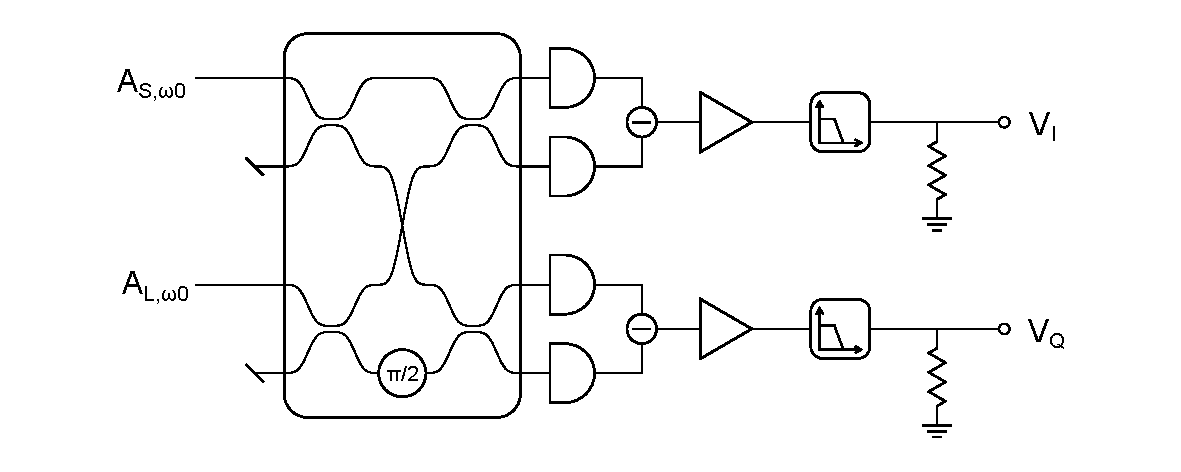
\includegraphics[width=15cm]{./sdf/optical_detection/figures/detection-IQ-balanced-homodyne.pdf}
	\caption{IQ balanced homodyne detection.}
\end{figure}
\noindent
{\bf \em Semiclassical model}\\
\\
{\bf \em Quantum model}\\


\paragraph{Heterodyne Detection}\ \\
%%
\begin{figure}[H]
	\centering
	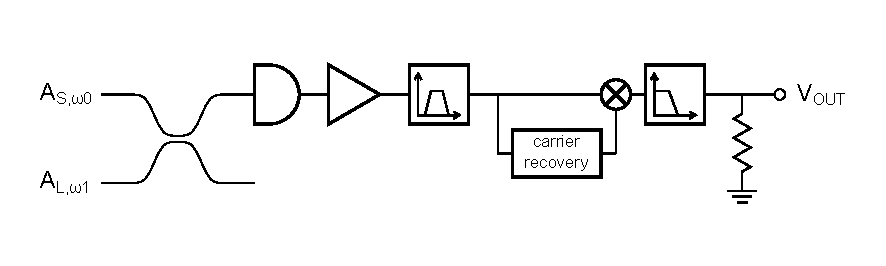
\includegraphics{./sdf/optical_detection/figures/detection-heterodyne.pdf}
	\caption{Heterodyne detection.}
\end{figure}

% inventado
In contrast with the homodyne detection, in which the frequency of the signal carrier is equal to the frequency of the local oscillator, in the heterodyne detection, these frequencies are different.\\
Because of this, the inference will result in a new signal with an intermediate frequency at...\\
% PROCURAR REFERENCIAS
\\



\paragraph{Balanced Heterodyne Detection}\ \\
%%
\begin{figure}[H]
	\centering
	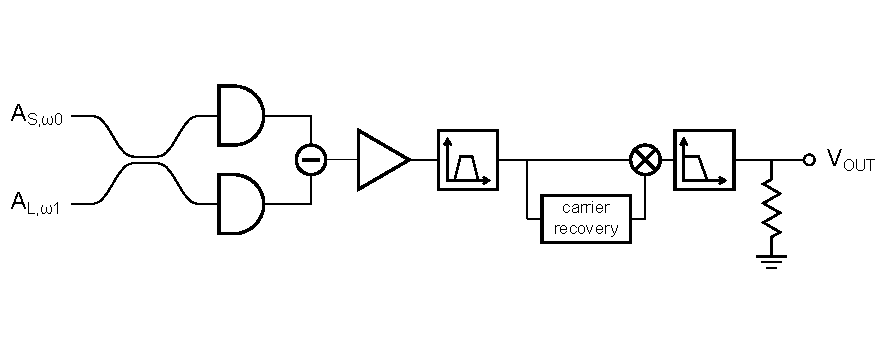
\includegraphics{./sdf/optical_detection/figures/detection-balanced-heterodyne.pdf}
	\caption{Balanced heterodyne detection.}
\end{figure}
%
\noindent
{\bf \em Semiclassical model}\\
\\
{\bf \em Quantum model}\\


\paragraph{IQ Heterodyne Balanced Detection}\ \\
%
\begin{figure}[H]
	\centering
	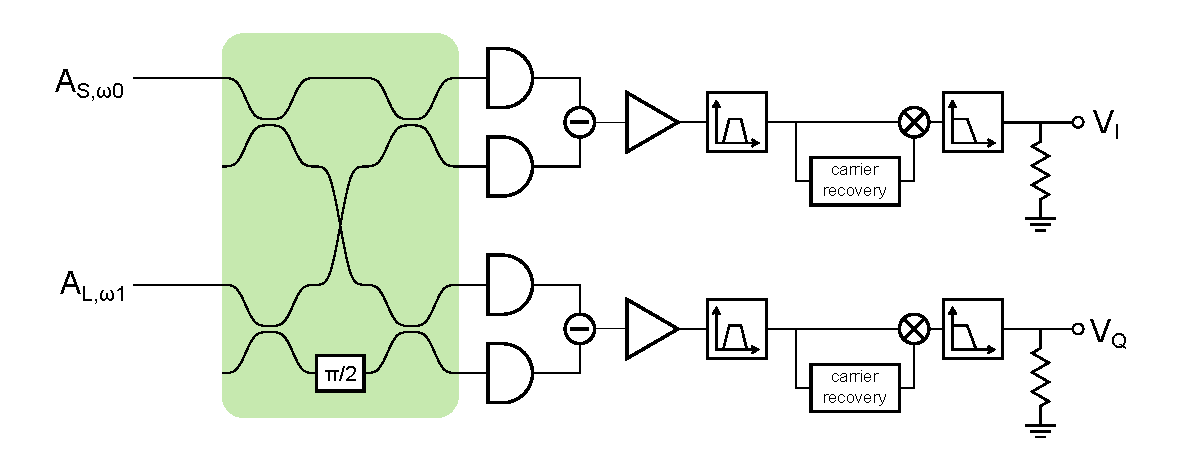
\includegraphics[width=15cm]{./sdf/optical_detection/figures/detection-IQ-balanced-heterodyne.pdf}
	\caption{IQ balanced heterodyne detection.}
\end{figure}
%
\noindent
\subsubsection{Thermal noise}
Thermal noise is generated by electrons in response to temperature. It's contribution to the resulting current can be described by the following equation
\cite{fox2006}
%\footnote{Mark Fox, p. 96}
%
\begin{equation}
\braket{(\Delta i_T)^2} = 4 K_B T_0 B/R_L
\end{equation}
%
in which $K_B$ it's Boltzmann's constant, $T_0$ is the absolute temperature, $B$ is the bandwidth and $R_L$ is the receiver load impedance. The $B$ value is imposed by default or chosen when the measurements are made, but the $R_L$ value is dependent in the internal setup of the various components of the detection system. Nevertheless, for simulation purposes, we can just introduce an experimental value.\\
\vspace{1cm}
%
%


\subsubsection{Quantum Description}

\begin{tcolorbox}	
\begin{tabular}{p{2.75cm} p{0.2cm} p{10.5cm}}
\textbf{Contributors}  &:& Diamantino Silva (2017-08-18 - ...)\\
                       &:& Armando Pinto (2017-08-15 - ...)\\
\textbf{Goal}          &:& Develop a quantum description of various optical detection schemes, and compare with the classical description.\\
\end{tabular}
\end{tcolorbox}

We start by defining number states $\ket{n}$ (or Fock states), which correspond to states with perfectly fixed number of photons
%\footnote{Loundon, p.184}
\cite{loudon2000}.
Associated to those states are two operators, the creation $\hat{a}^\dagger$ and annihilation $\hat{a}$ operators, which in a simple way, remove or add one photon from a given number state
%\footnote{Mark Fox, p.155}
\cite{fox2006}.
Their action is defined as
%
\begin{center}
	\hspace{-4mm}
	\begin{minipage}{44mm}
		\noindent
		\begin{equation}
			\hat{a} \ket{n} = \sqrt{n} \ket{n-1}
		\end{equation}
	\end{minipage}
	$,\quad$
	\begin{minipage}{52mm}
		\noindent
		\begin{equation}
			\hat{a}^\dagger \ket{n} = \sqrt{n+1} \ket{n+1}
		\end{equation}
	\end{minipage}
	$,\quad$
	\begin{minipage}{35mm}
		\noindent
		\begin{equation}
			\hat{n} \ket{n} = n \ket{n}
		\end{equation}
	\end{minipage}
\end{center}
%
in which $\hat{n} = \hat{a}^\dagger\hat{a}$ is the number operator. Therefore, number states are eigenvectors of the number operator.\\
\\
Coherent states have properties that closely resemble classical electromagnetic waves, and are generated by single-mode lasers well above the threshold.
\cite{loudon2000}
%\footnote{Loudon, p.190}
We can defined them, using number states in the following manner
\begin{equation}
\ket{\alpha} = e^{-\frac{|\alpha|^2}{2}} \sum_{n=0}^\infty \frac{\alpha^n}{\sqrt{n!}} \ket{n}
\end{equation}
in which the complex number $\alpha$ is the sole parameter that characterizes it.
%\footnote{Loudon, p.184}
%\footnote{Loudon, p.186}
In fact, if we calculate the expected number of photons with $\bra{\alpha} \hat{n} \ket{\alpha}$ we will obtain $|\alpha|^2$. The coherent state is an eigenstate of the annihilation operator, $\hat{a}\ket{\alpha} = \alpha \ket{\alpha}$.\\
\\
%
%
Using the creation and annihilation operators, we can define two quadrature operators
\cite{loudon2000}
%\footnote{Loudon, p.138, (4.3.36)}
%
\begin{center}
	\begin{minipage}{41mm}
		\noindent
		\begin{equation}
			\hat{X} = \frac{1}{2} \left( \hat{a}^\dagger + \hat{a} \right)
		\end{equation}
	\end{minipage}
	$,\quad$
	\begin{minipage}{40mm}
		\noindent
		\begin{equation}
			\hat{Y} = \frac{i}{2} \left( \hat{a}^\dagger - \hat{a} \right)
		\end{equation}
	\end{minipage}
\end{center}
%
The expected value of these two operators, using a coherent state $\ket{\alpha}$ are
%
\begin{center}
	\begin{minipage}{37mm}
		\noindent
		\begin{equation}
			\braket{\hat{X}} = \textrm{Re}(\alpha)
		\end{equation}
	\end{minipage}
	$,\quad$
	\begin{minipage}{37mm}
		\noindent
		\begin{equation}
			\braket{\hat{Y}} = \textrm{Im}(\alpha)
		\end{equation}
	\end{minipage}
\end{center}
%
We see that the expected value of these operators give us the real and imaginary part of $\alpha$. Now, we can obtain the uncertainty of these operators, using:
%
\begin{equation}
\textrm{Var}(\hat{X}) = \braket{\hat{X}^2} - \braket{\hat{X}}^2
\end{equation}
%
For each of these quadrature operators the variance will be
%
\begin{equation}
\textrm{Var}(\hat{X}) = \textrm{Var}(\hat{Y}) = \frac{1}{4}
\end{equation}
%
This result show us that for both quadratures, the variance of measurement is the same and independent of the value of $\alpha$.
%
%
%
\subsubsection{Homodyne detection}

The measurent of a quadrature of an input signal (S) is made by using the balanced homodyne detection technique, which measures the phase difference between the input signal and a local oscillator (LO). The measurement of quadrature are made relative to a reference phase of the LO, such that if the measurement is made in-phase with this reference, the value will be proportional to the $\hat{X}$ quadrature of the signal. If the phase of the LO is has an offset of $\pi/2$ relative to the reference, the output will be proportional to the $\hat{Y}$ quadrature of the signal.\\
\\
Experimentally, the balanced homodyne detection requires a local oscillator with the same frequency as the input signal, but with a much larger amplitude. These two signals are combined using a 50:50 beam splitter, from were two beams emerge, which are then converted to currents using photodides. Finally, the two currents are subtracted, resulting in an output current proportional to a quadrature of the input signal
\cite{fox2006}.\\
%\footnote{Mark Fox, p. 140}
%
%The balanced homododyne technique is used to measure the phase of the input signal (S), relative to the phase of a local oscillator (LO), which has the same frequency as the input signal, but a much larger amplitude. The technique consists in combining the input signal and the local oscillator, using a 50:50 beam splitter, from whom two beams emerge, which are then converted to currents using photodides. Finally, the two currents are subtracted, resulting in an output current.\\
A phase of the local oscillator can be defined as the reference phase. A phase offset equal to $0$ or $\pi/2$ will give an output proportional to the signal's in-phase component or to the quadrature component, respectively. Therefore, the $\hat{X}$ operator will correspond to the in-phase component and $\hat{Y}$ operator correspond to quadrature component
%\cite{fox2006}.
%\footnote{Mark Fox, p. 140}
\\
%
\begin{figure}[H]
	\label{fig:scheme_homodyne}
	\centering
	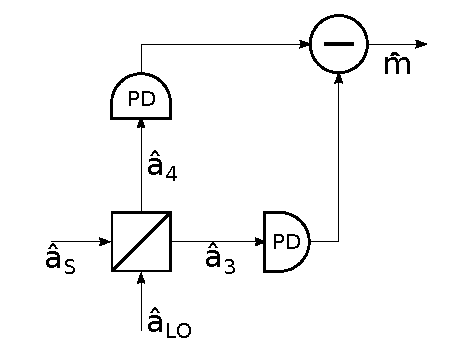
\includegraphics{./sdf/optical_detection/figures/scheme_homodyne.pdf}
	\caption{Balanced homodyne detection.}
\end{figure}
%
In the lab and in our simulations, a more complex system is used, the double balanced homodyne detection, which allows the simultaneous measurement of the $\hat{X}$ and $\hat{Y}$ components. The signal is divided in two beam with half the power of the original. One of the beams is used in a balanced homodyne detection with a local oscillator. The other beam is used in another balanced homodyne detection, but using a local oscillator with a phase difference $\pi/2$ relative to the first one.
%
\begin{figure}[H]
	\label{fig:scheme_homodyne}
	\centering
	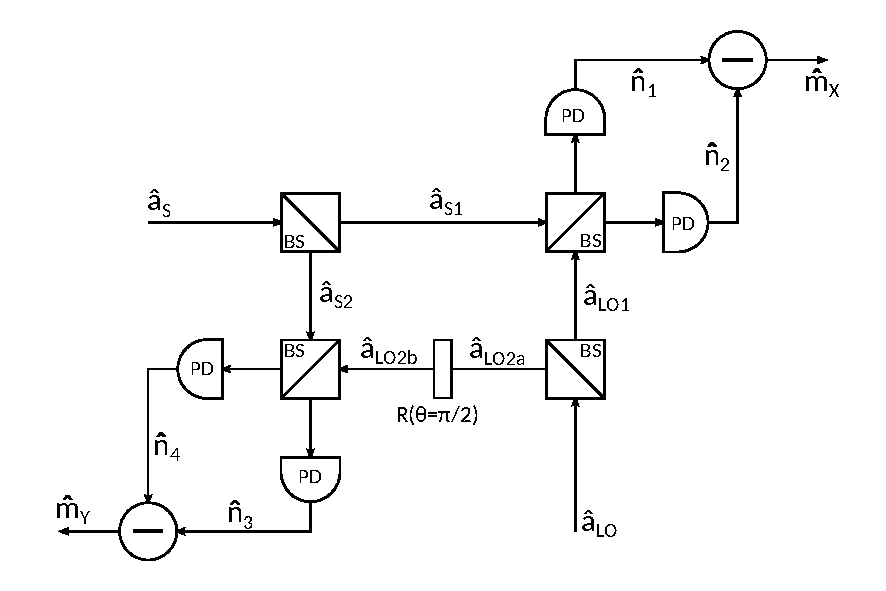
\includegraphics{./sdf/optical_detection/figures/scheme_double_homodyne.pdf}
	\caption{Balanced double homodyne detection.}
\end{figure}
%
%
%

\begin{thebibliography}{10}

\bibitem{Kahn2006}
  Joseph M. Kahn,
  \textit{Modulation and Detection Techniques for
Optical Communication Systems},
  OSA/COTA -  Coherent Optical Technologies and Applications Topical Meeting, BC, Canada,
  2006.
  \bibitem{Kahn2004}
  Joseph M. Kahn, and Keang-Po Ho,
Spectral Efficiency Limits and Modulation/Detection
Techniques for DWDM Systems,
  \textit{IEEE Journal Of Selected Topics In Quantum Electronics}, Vol. 10, No. 2, 2004.

\end{thebibliography}

\subsubsection{Noise sources in homodyne detection}
The detection of light using photodiodes is subjected to various sources of noise. One of these sources is the electrical field itself. The interaction of the signal with the vaccuum field adds quantum noise to the detection.
Another source of noise comes from the detection system, such as photodiodes and other electrical circuits, originating various kinds of noise, such as thermal noise, dark noise and amplifier noise
%\footnote{Hans, p.185}
\cite{hans2004}.
In the following sections, we will focus on two noise sources, quantum noise and thermal noise.
%
%
%
\subsubsection{Quantum Noise}
In order to grasp this effect, the quantum mechanical description of balanced homodyne detection will be used, employing quantum operators to describe the effect of each component in the system (fig. \ref{fig:scheme_homodyne}). We start with the operators $\hat{a}_S$ and $\hat{a}_{LO}$ corresponding to the annihilation operator for the signal and local oscillator, which are the inputs in a beam divisor. The outputs will be $\hat{a}_3$ and $\hat{a}_4$.
Using a balanced beam splitter, we can write the output as
%
\begin{center}
	\begin{minipage}{48mm}
		\noindent
		\begin{equation}
			\hat{a}_3 = \frac{1}{\sqrt{2}} \left( \hat{a}_S + \hat{a}_{LO} \right)
		\end{equation}
	\end{minipage}
	$,\quad$
	\begin{minipage}{48mm}
		\noindent
		\begin{equation}
			\hat{a}_4 = \frac{1}{\sqrt{2}} \left( \hat{a}_S - \hat{a}_{LO} \right)
		\end{equation}
	\end{minipage}
\end{center}
%
The final output of a homodyne measurement will be proportional to the difference between the photocurrents in arm $3$ and $4$. Then
%
\begin{equation}
I_{34} = I_3 - I_4 \sim \braket{\hat{n}_3 - \hat{n}_4}
\end{equation}
%
We can define an operator that describes the difference of number of photons in arm 3 and arm 4:
%
\begin{equation}
\hat{m} = \hat{a}^\dagger_3\hat{a}_3 - \hat{a}^\dagger_4\hat{a}_4
\end{equation}
%
If we assume that the local oscillator produces the the coherent state $\ket{\beta}$, then the expected value of this measurement will be
%
\begin{center}
	\begin{minipage}{58mm}
		\noindent
		\begin{equation}
			\braket{m} = 2|\alpha||\beta|\cos({\theta_\alpha - \theta_\beta})
		\end{equation}
	\end{minipage}
	$,\quad$
	\begin{minipage}{46mm}
		\noindent
		\begin{equation}
			\textrm{Var}(m) = |\alpha|^2 + |\beta|^2
		\end{equation}
	\end{minipage}
\end{center}
%
The local oscillator normally has a greater power than the signal
%VER REFERENCIAS
, then $|\alpha| \ll |\beta|$. If we use as unit, $2|\beta|$, then these two quantities can be simplified to
%
\begin{center}
	\begin{minipage}{52mm}
		\noindent
		\begin{equation}
			\label{eq:var_m}
			\braket{m} = |\alpha|\cos({\theta_\alpha - \theta_\beta})
		\end{equation}
	\end{minipage}
	$,\quad$
	\begin{minipage}{34mm}
		\noindent
		\begin{equation}
			\textrm{Var}(m) \approx \frac{1}{4}
		\end{equation}
	\end{minipage}
\end{center}
%
\cite{hans2004}
%\footnote{Referencia indirecta: Livro: Hans, p.207}
\\
Has we have seen previously, in order to measure two quadratures simultaneously, we can use double balanced homodyne detection. For each quadrature, the input signal now has half the power, so $|\alpha| \rightarrow |\alpha/\sqrt{2}|$.  If we use a local oscillator that produces states $\ket{\beta}$, then we can divide it in two beams in state $\ket{\beta/\sqrt{2}}$ and $\ket{i\beta/\sqrt{2}}$ which will be used in each homodyne detection. In this setting, the expected values for each quadrature, $X$ and $Y$, (in normalized values of $\sqrt{2}|\beta|$) are
%
\begin{center}
	\begin{minipage}{58mm}
		\noindent
		\begin{equation}
			\braket{m_X} = \left|\frac{\alpha}{\sqrt{2}}\right| \cos({\theta_\alpha - \theta_\beta})
		\end{equation}
	\end{minipage}
	$,\quad$
	\begin{minipage}{37mm}
		\noindent
		\begin{equation}
			\textrm{Var}(m_X) \approx \frac{1}{4}
		\end{equation}
	\end{minipage}
\end{center}
%
%
\begin{center}
	\begin{minipage}{58mm}
		\noindent
		\begin{equation}
			\braket{m_Y} =  \left|\frac{\alpha}{\sqrt{2}}\right| \sin({\theta_\alpha - \theta_\beta})
		\end{equation}
	\end{minipage}
	$,\quad$
	\begin{minipage}{37mm}
		\noindent
		\begin{equation}
			\textrm{Var}(m_Y) \approx \frac{1}{4}
		\end{equation}
	\end{minipage}
\end{center}
%
Therefore the measurement of each quadrature will have half the amplitude, but the same variance.
%
%
%

